\section{Trigger Studies} %updated May 15 2017
\label{app:trig}

\paragraph{} This appendix is complimentary to section~\ref{evt-sel:trig}. In order to check different trigger efficiencies, trigger efficiency as a function of signal mass are shown. 

\paragraph{} For 2016 run, the lowest unprescaed large-$R$ jet trigger is \verb|HLT_j420_a10_lcw_L1J100|, see \href{https://twiki.cern.ch/twiki/bin/viewauth/Atlas/LowestUnprescaled}{Twiki link}. LCW cluster trigger is chosen, since the other option, reclusted large-$R$ jet trigger, has slower turn-on in QCD events. The lowest unprescaled HT trigger, \verb|HLT_ht1000|, is also tested. HT trigger has a much slower turn-on compared to large-$R$ jet triggers. Another trigger shown is \verb|HLT_4j100|, and because of the boosted jets merging, this trigger efficiency decreases rapidly as the signal mass increases. The trigger efficiency relative to all events or only events passing the large-$R$jet selections are shown in Figure~\ref{fig:app-trig-eff-mass}.

\begin{figure*}[htbp!]
\begin{center}
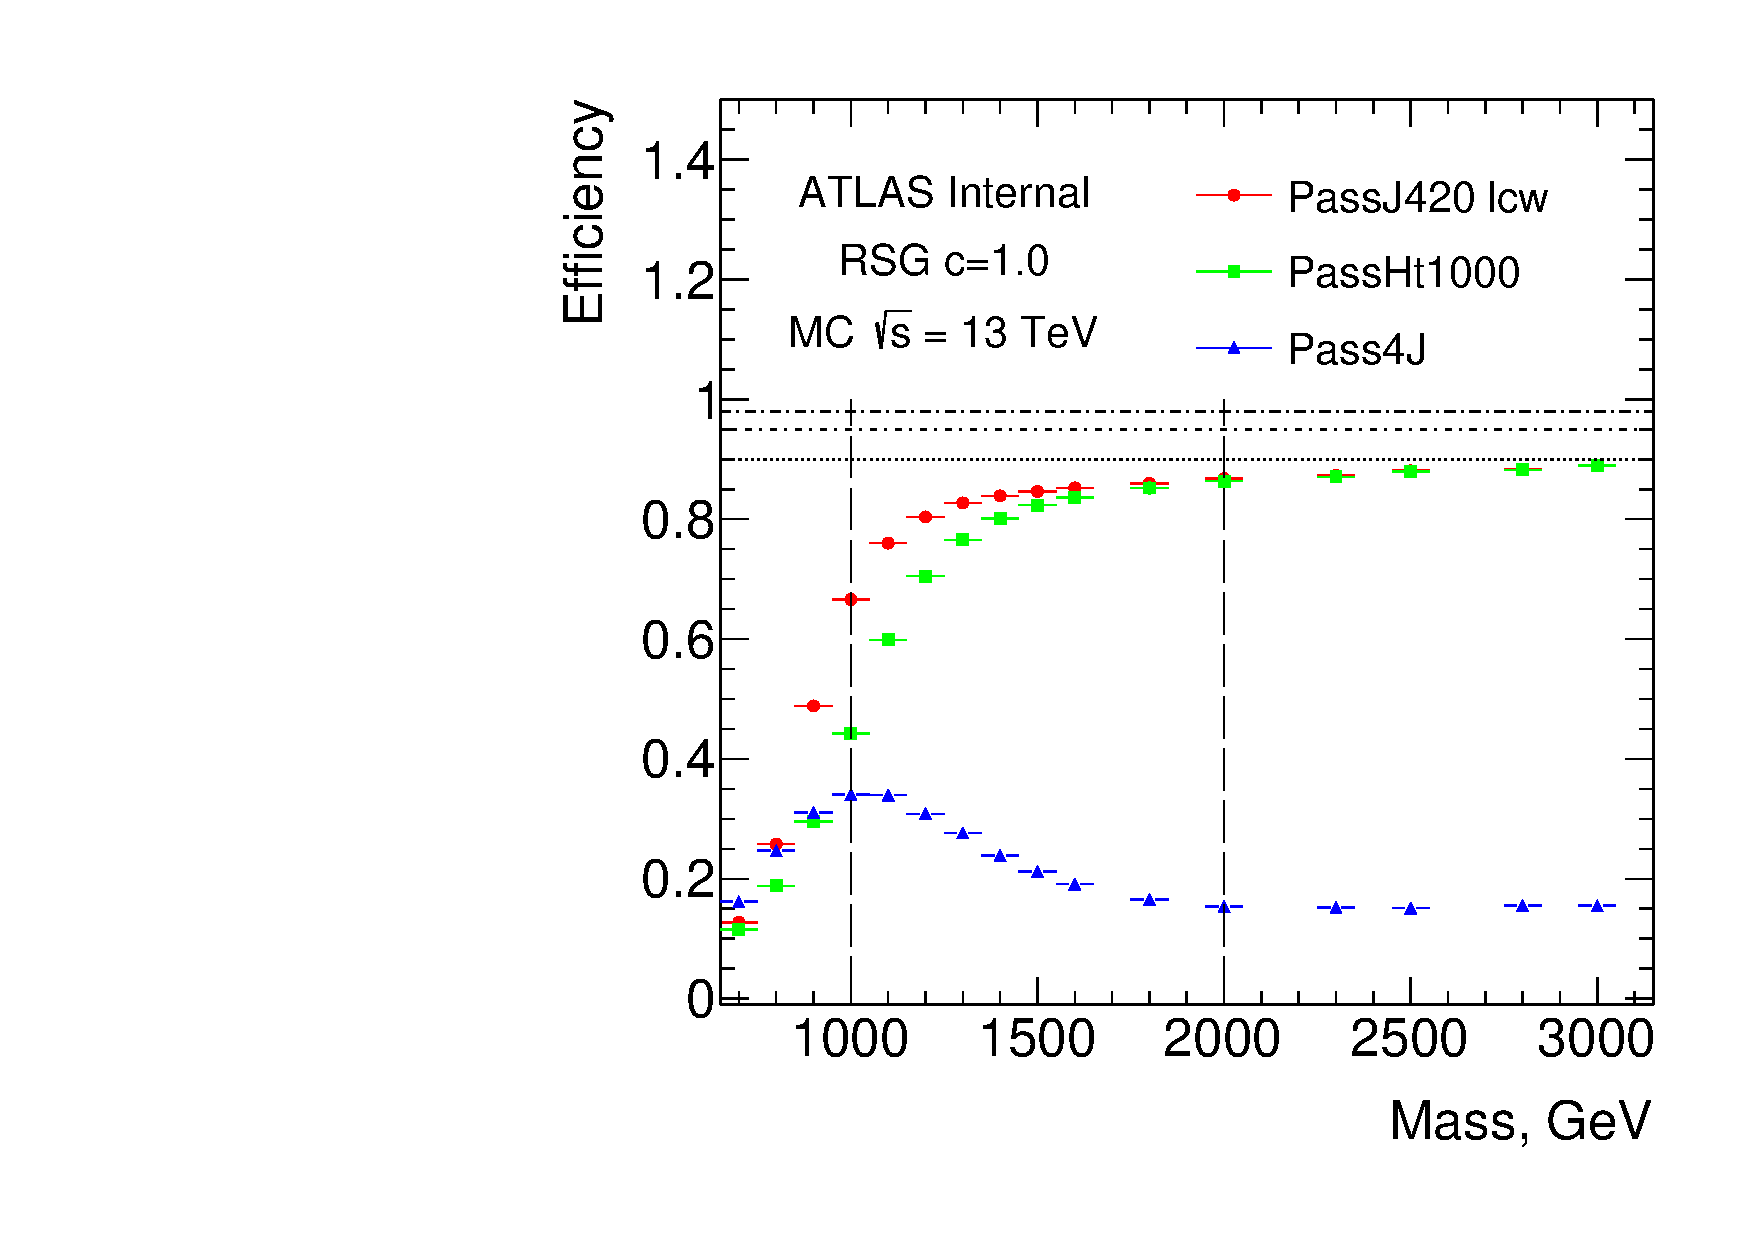
\includegraphics[angle=270, width=0.45\textwidth]{./figures/boosted/Trigger/app_trig_b77_Efficiency_PreSel.pdf}
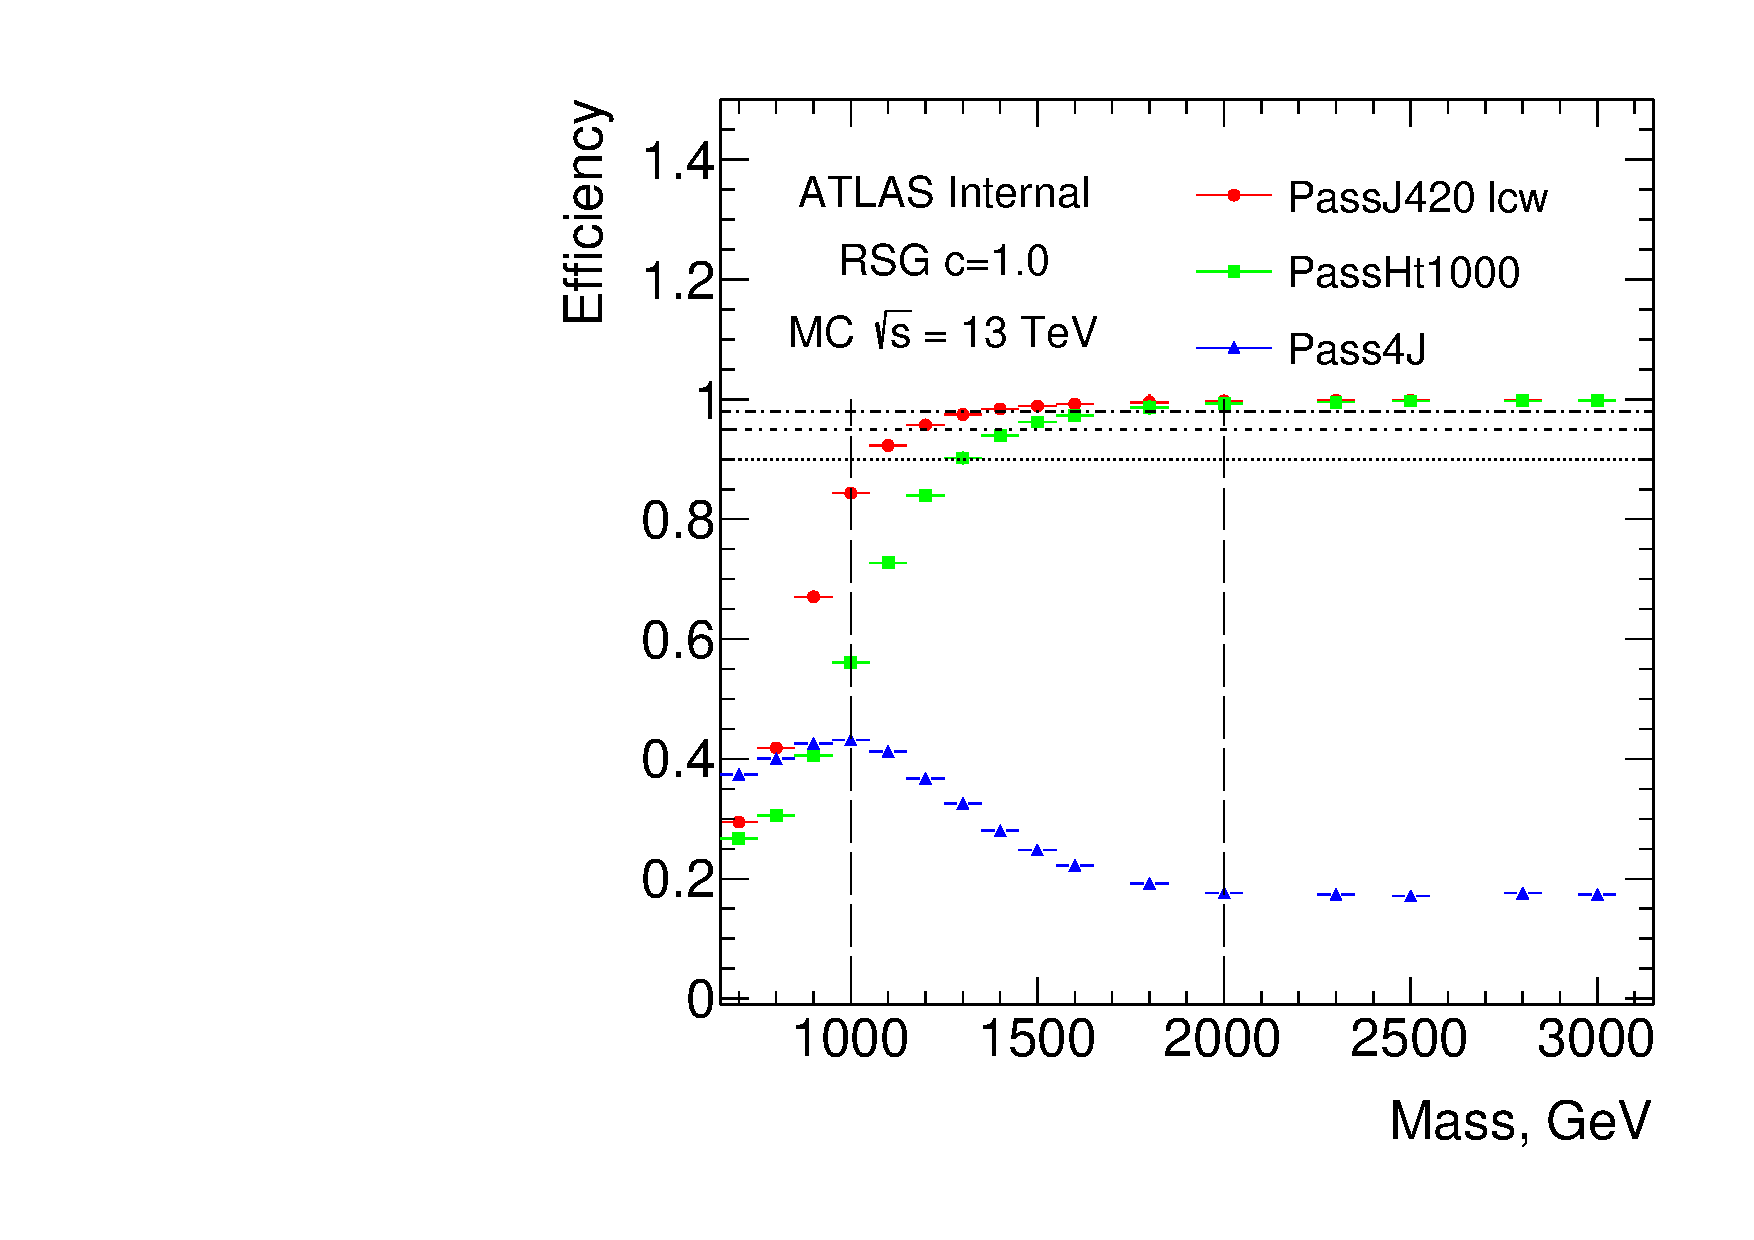
\includegraphics[angle=270, width=0.45\textwidth]{./figures/boosted/Trigger/app_trig_b77_Efficiency_All.pdf}
  \caption{Trigger efficiencies as a function of the signal resonance mass with respect to all events with no selection (left) and with respect to events passing the two large-$R$ jets requirement and leading/subleading jet $p_{T}$ requirement (right). }
\label{fig:app-trig-eff-mass}
\end{center}
\end{figure*}

\paragraph{} To further test if a combination of triggers will improve the seleciton efficiency, events passing either one of the three triggers (\verb|HLT_j420_a10_lcw_L1J100|, \verb|HLT_ht1000|, \verb|HLT_4j100|) are compared with the trigger \verb|HLT_j420_a10_lcw_L1J100|, see Figure~\ref{fig:app-trig-releff-mass}. The combined trigger shows only a small gain compared with the single trigger, while requiring fsignal MC events passing the signal region selection. The gain is around $2-4\%$, for signal resonance mass less than 1 TeV only. Therefore, the trigger \verb|HLT_j420_a10_lcw_L1J100| is kept as the only trigger used in the selection.

\begin{figure*}[htbp!]
\begin{center}
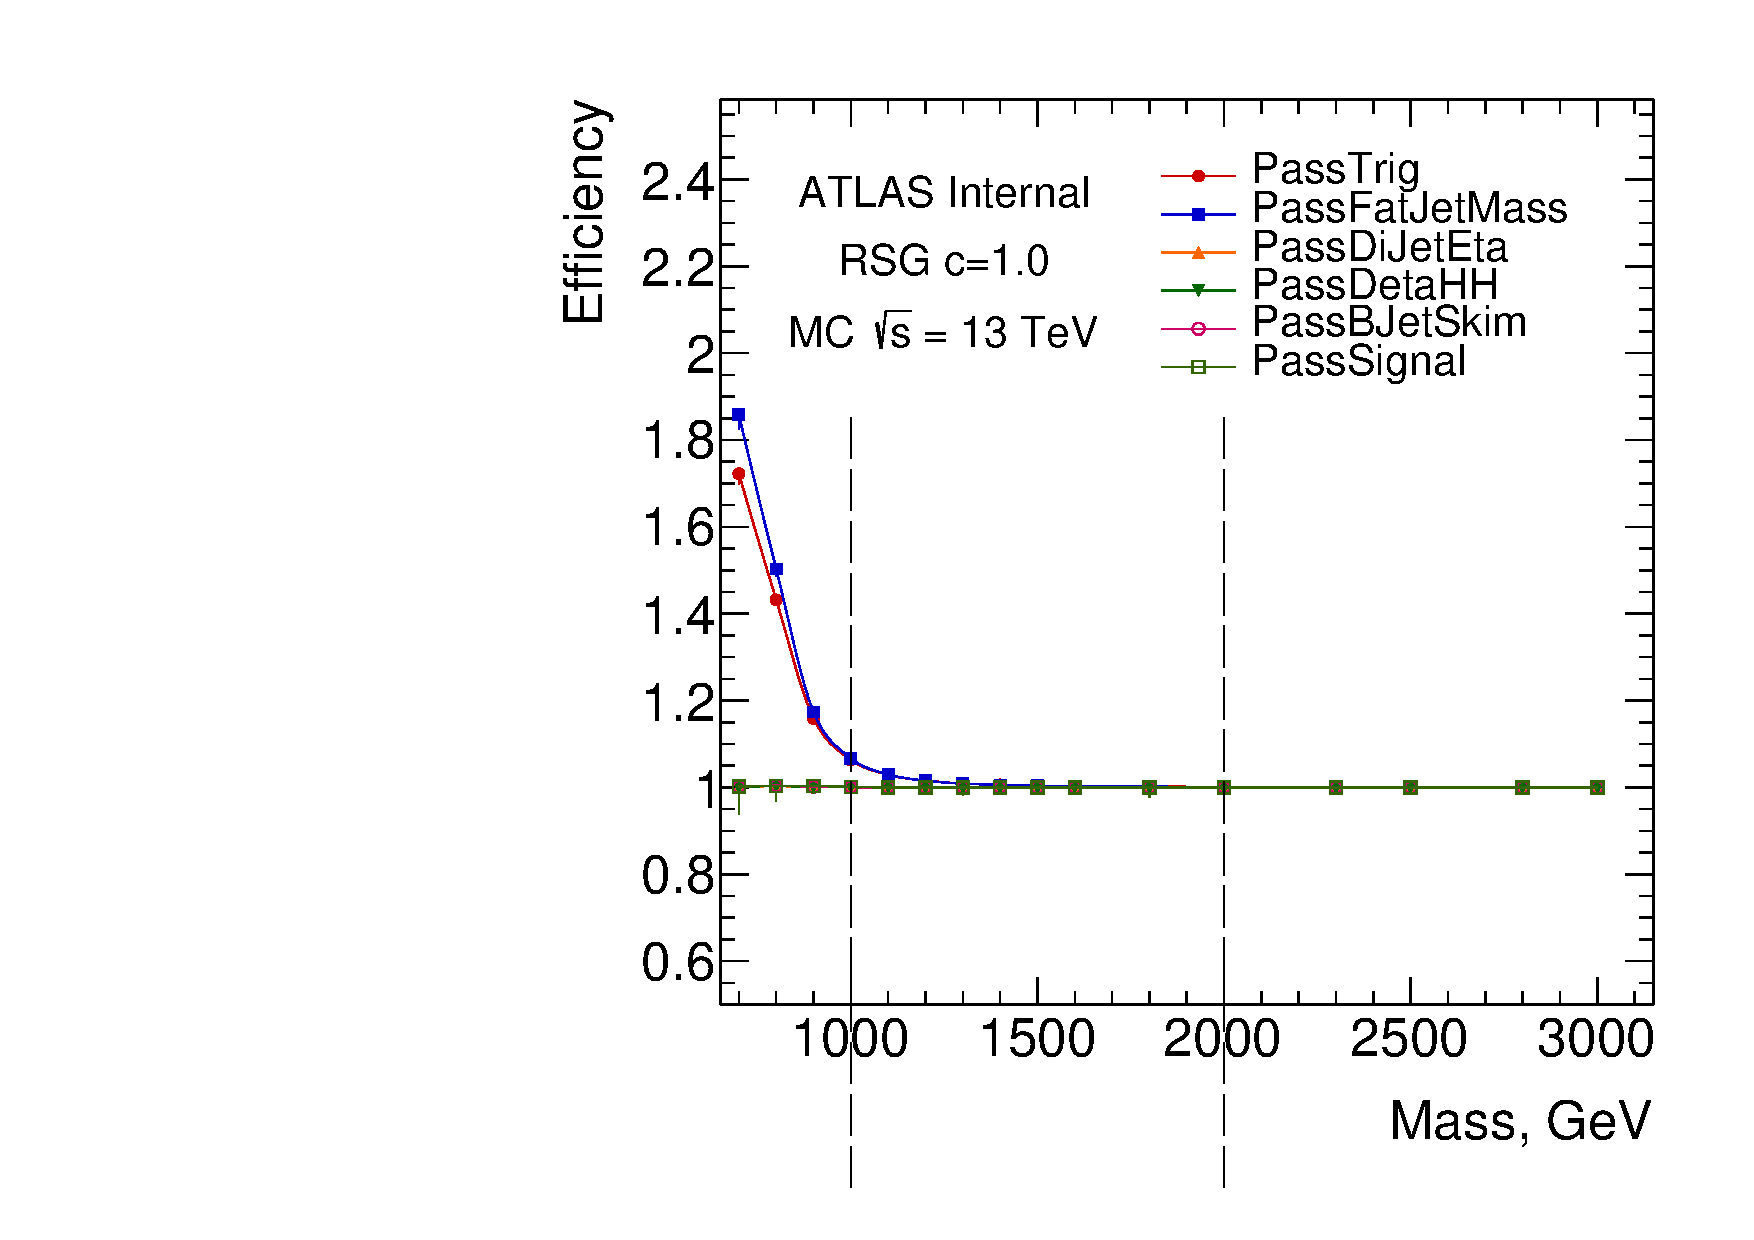
\includegraphics[angle=270, width=0.45\textwidth]{./figures/boosted/Trigger/evtsel_test_noveto_Efficiency_All_ref_full.pdf}
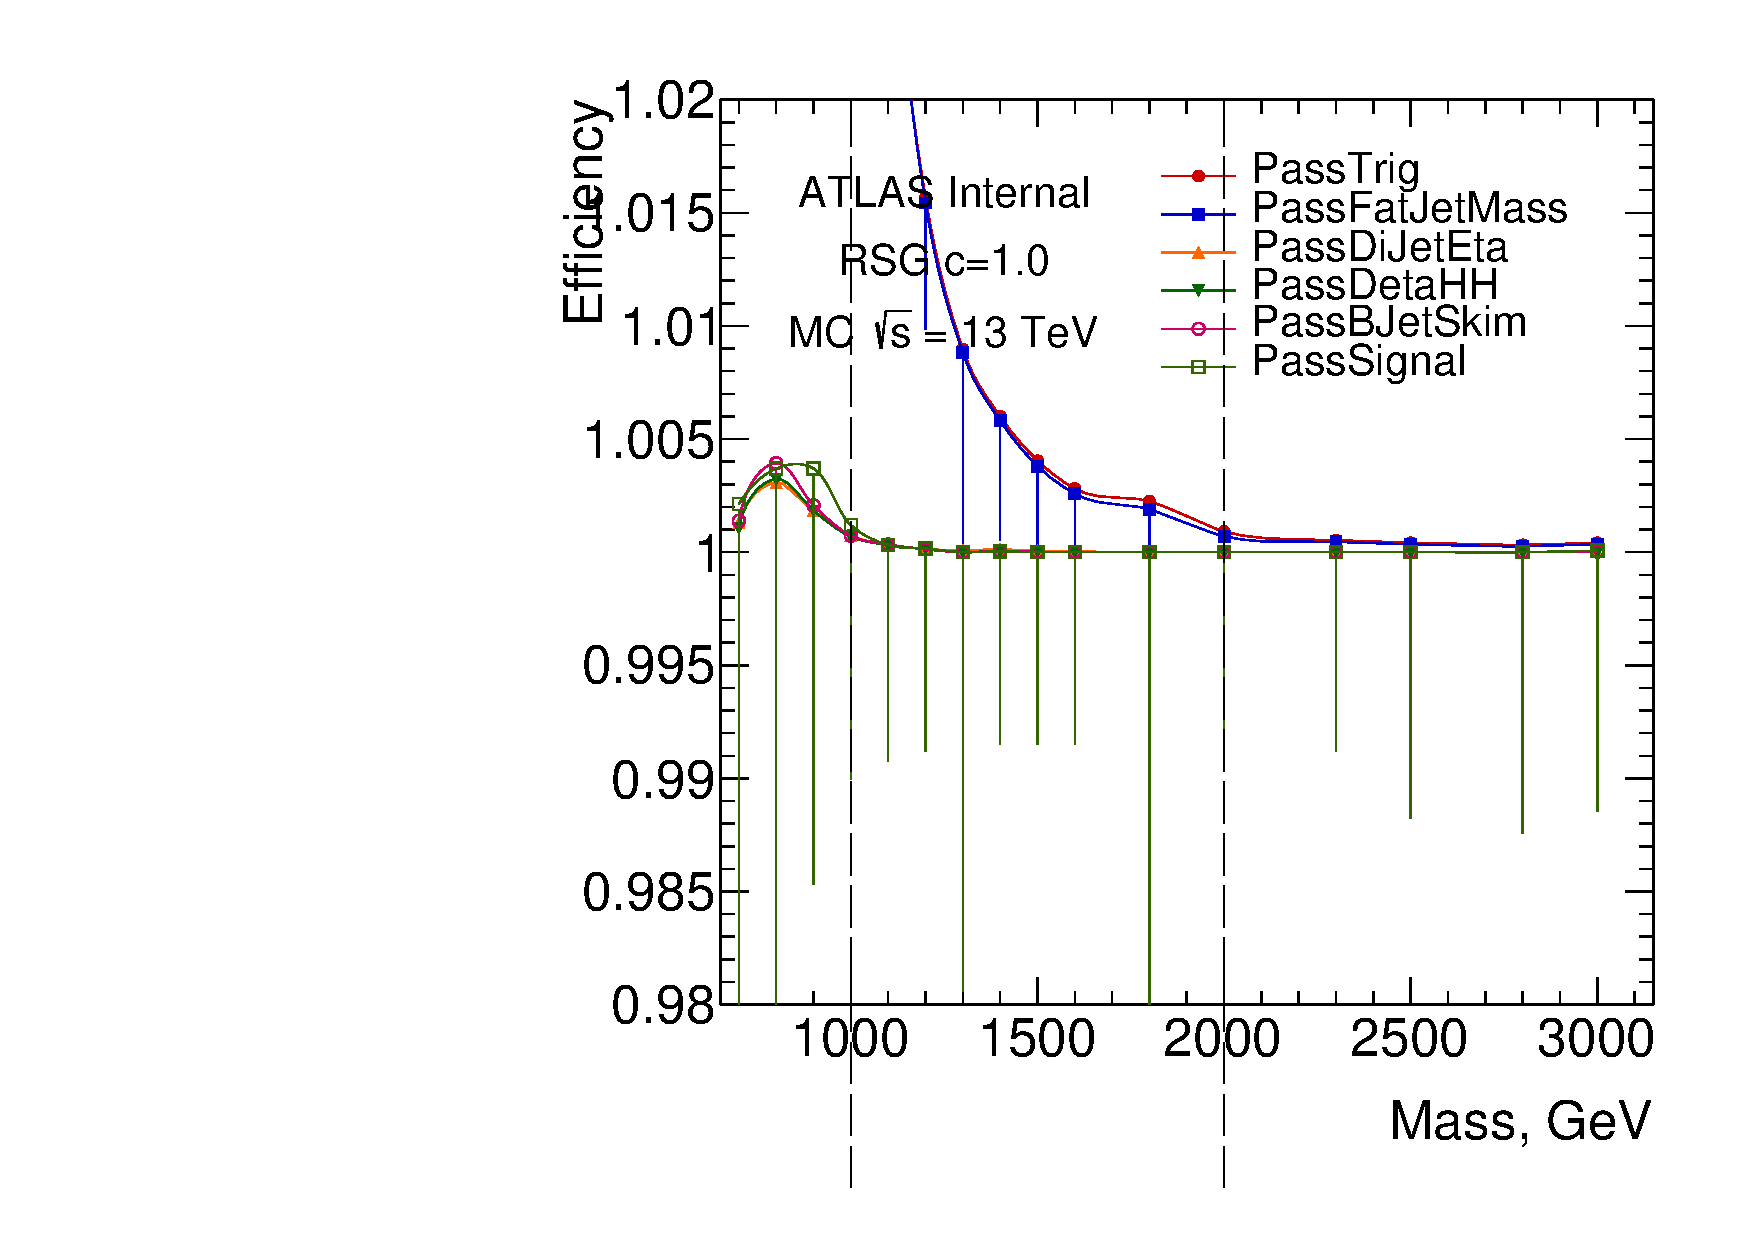
\includegraphics[angle=270, width=0.45\textwidth]{./figures/boosted/Trigger/evtsel_test_noveto_Efficiency_All_ref_zoom.pdf}
  \caption{Relative ratio between the efficiency using the combined trigger and the efficiency using the single trigger as a function of the signal resonance mass with respect to all events with no selection (left) and zoomed in on the efficiency range (right). The trigger selection effiency is improved when using the combined trigger, however, the effect on the number of events passing the signal region is less than $1\%$ for resonance mass above 1 TeV.}
\label{fig:app-trig-releff-mass}
\end{center}
\end{figure*}
